\chapter{The Dataset}
\label{ch:dataset}

The dataset used in this project is the \textit{AI-ArtBench} dataset from Kaggle \cite{aiartbench}.
It contains over $180000$ images, of which $60000$ are human drawn and the rest are AI generated.
The images are pre-split into train and test data, with around $155015$ and $30000$ used for training and testing, respectively.
Further, the dataset is divided into different subfolders, each containing images from a different epoch.
Those epochs are: Art Nouveau, Baroque, Expressionism, Impressionism, Post impressionism, Realism, Renaissance, Romanticism, Surrealism, Ukiyo-e. \\

It should be noted that the AI generated images in this dataset were generated using two different models, Latent Diffusion (LD) and Standard Diffusion (SD).
The exact machinations of those models are not relevant here, nor is it our aim to differentiate between them.
Thus, the AI generated images were thrown together into a single category.
Another minor change made to the dataset was to cap all folder at $5000$ images, at least before fusing the LD and SD folders.
This is the number of images for the folders containing the human drawn art.
While the inconsistency in the number of images per epoch was minute, we thought it sufficient to sacrifice a few images for the sake of stability.
Additionally, some images had to be resized, as, contrary to what the dataset's description claims, some images were indeed not square $256 \times 256$ images,
but rectangular instead.
Those images were cropped to $256 \times 256$ pixels. \\

\begin{figure}
    \centering
    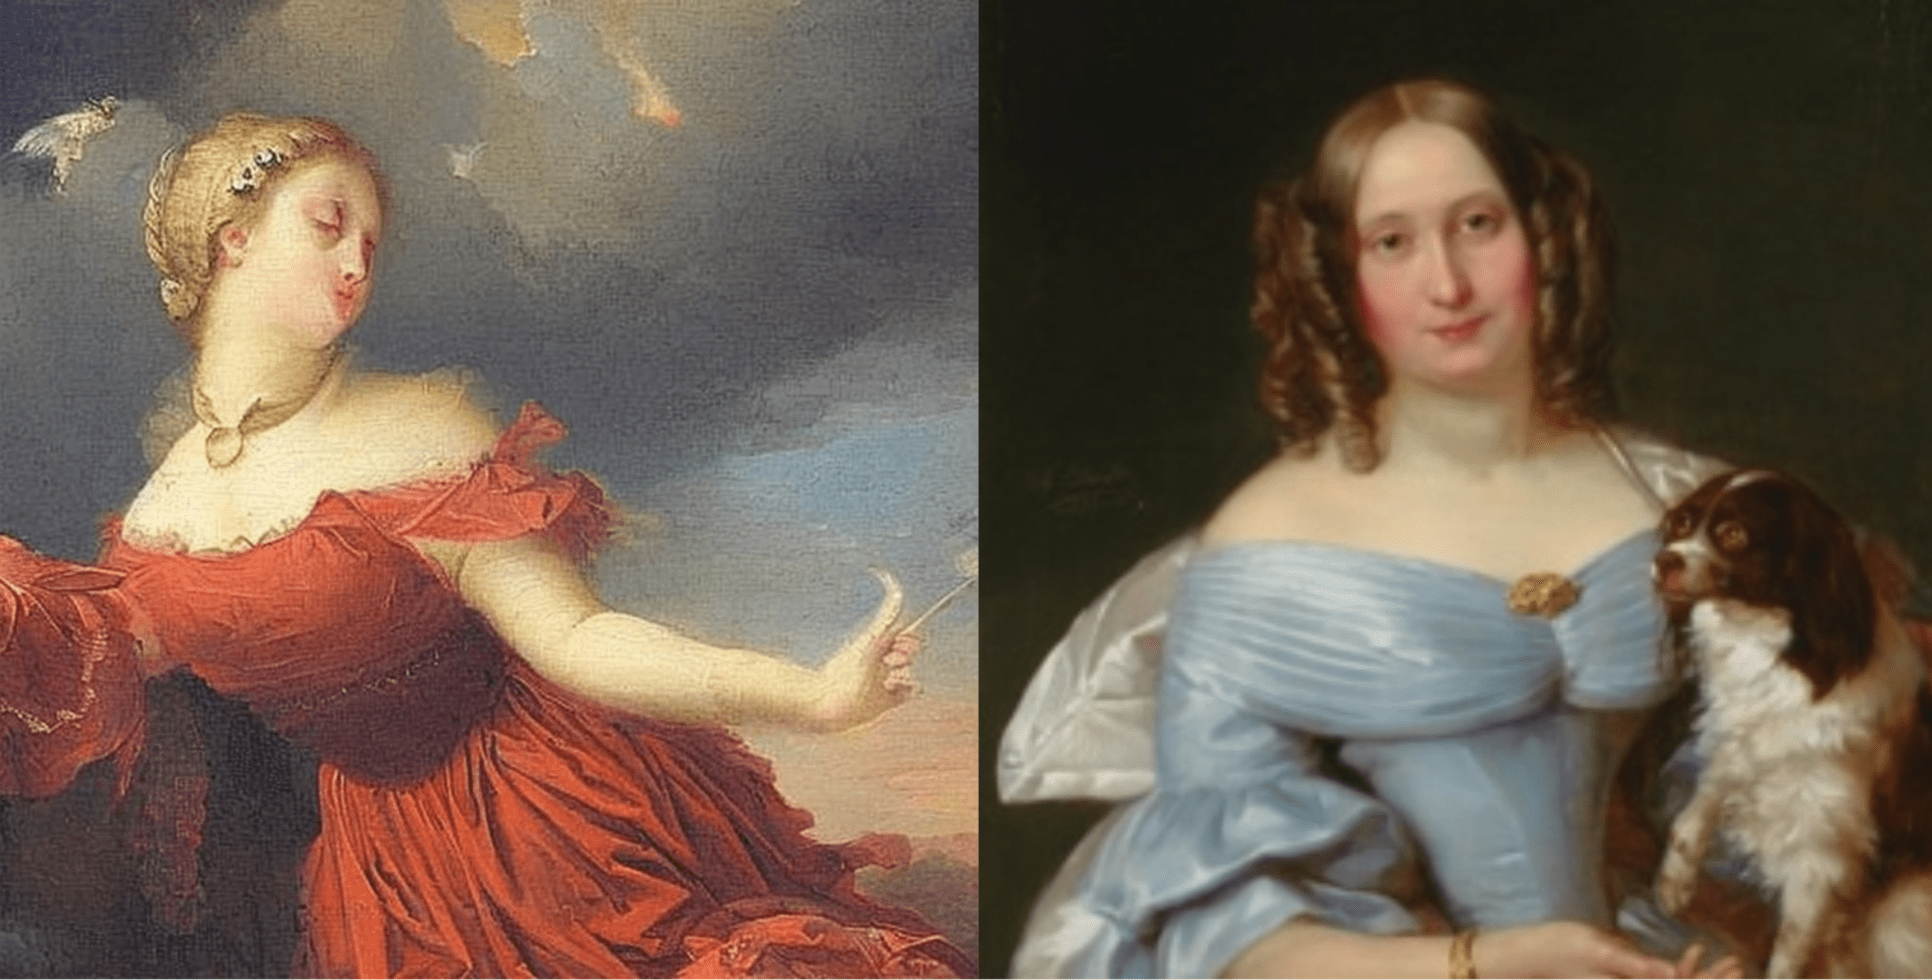
\includegraphics[width=0.5\textwidth]{images/Example_images.png}
    \caption{Example images from the dataset with the AI generated image on the left and the human-drawn on the right \cite{aiartbench}.}
    \label{fig:example_images}
\end{figure}

Concerning previous work, we found one work on this exact dataset by Kaggle user \textit{nibrastuhh} \cite{useraiartbench}, who used
a neural network to classify the images, reaching an accuracy of over $90\%$.
They, however, focused on merely the classification of the images, while we are going to be focusing more on the details.
Typically, other work in the same direction focuses on detecting AI generated photographs, not art.

